\documentclass{beamer}
\usepackage{extras}
\usetheme{default}
\usecolortheme{dove}
\usepackage{lmodern}
\title{Konstruktion av en autonom undsättningsrobot}
\subtitle{Kandidatprojekt i elektronik vid Linköpings universitet}
\author{Grupp 4}
\beamertemplatenavigationsymbolsempty
\date{\today}

\begin{document}

\begin{frame}
  \titlepage
\end{frame}


\begin{frame}{PigBot}
  \begin{columns}
    \begin{column}{0.5\textwidth}
      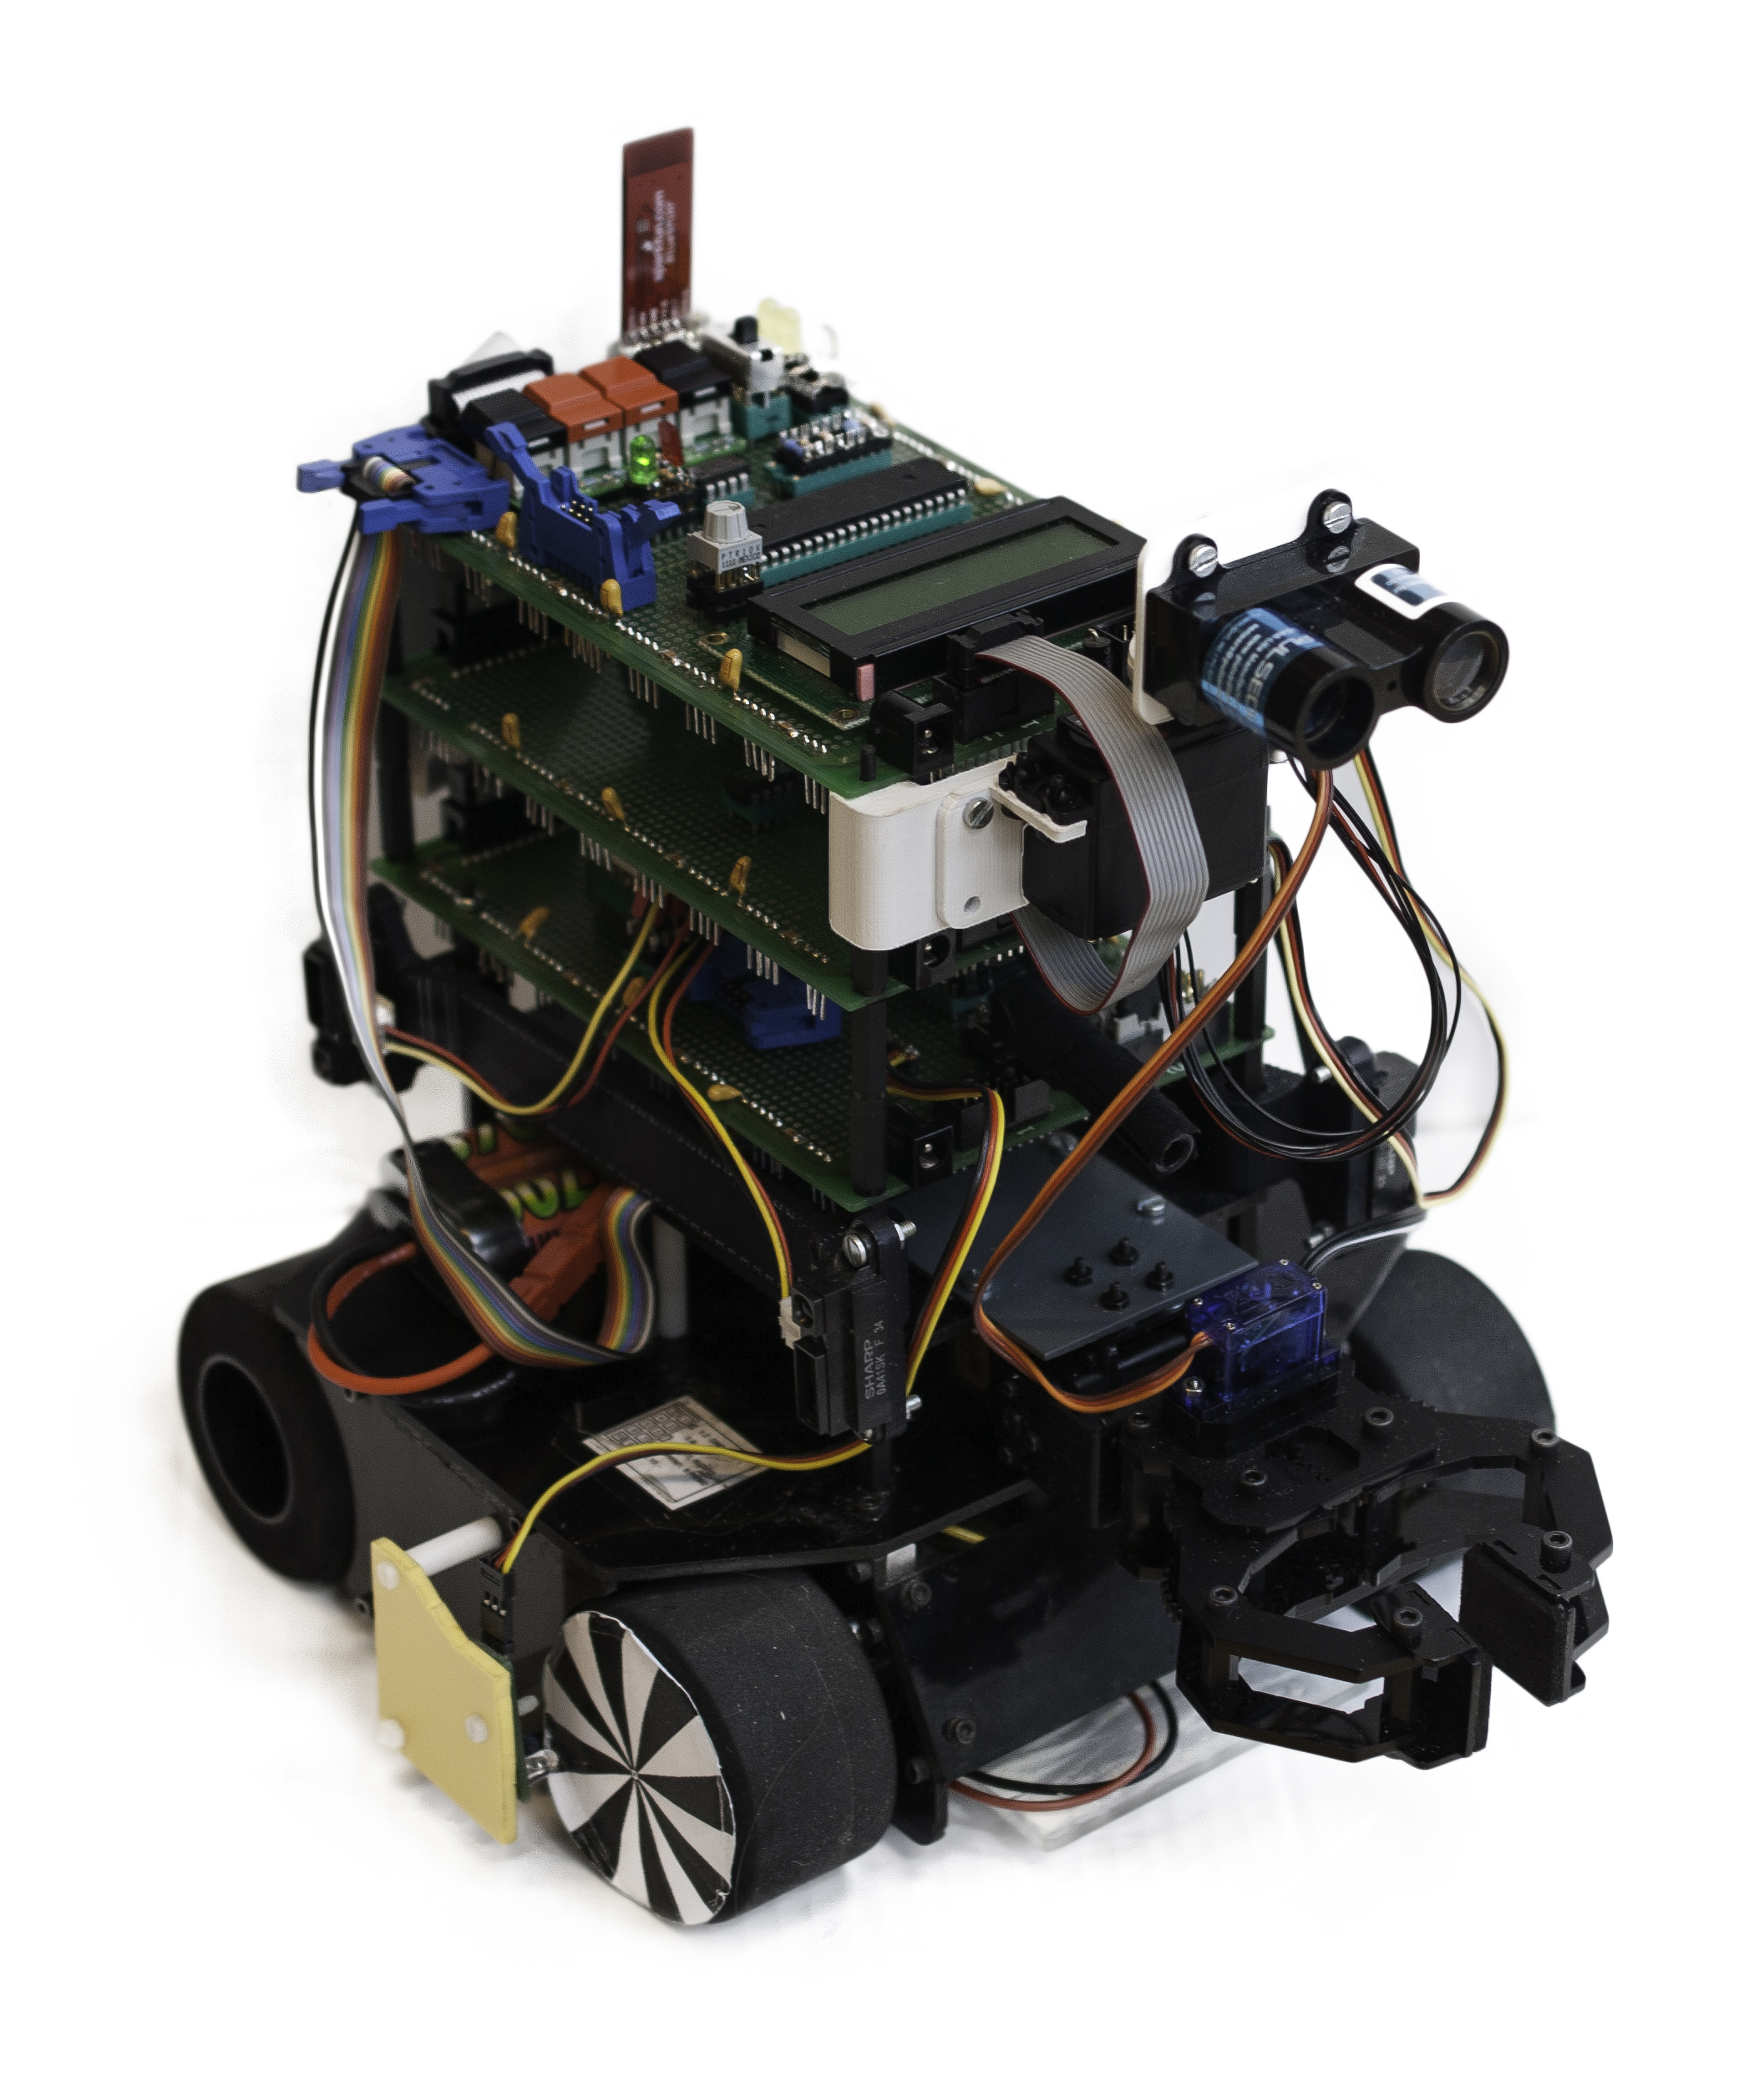
\includegraphics[width=0.9\textwidth]{images/RobotFront.pdf}
    \end{column}%
    \begin{column}{0.5\textwidth}
      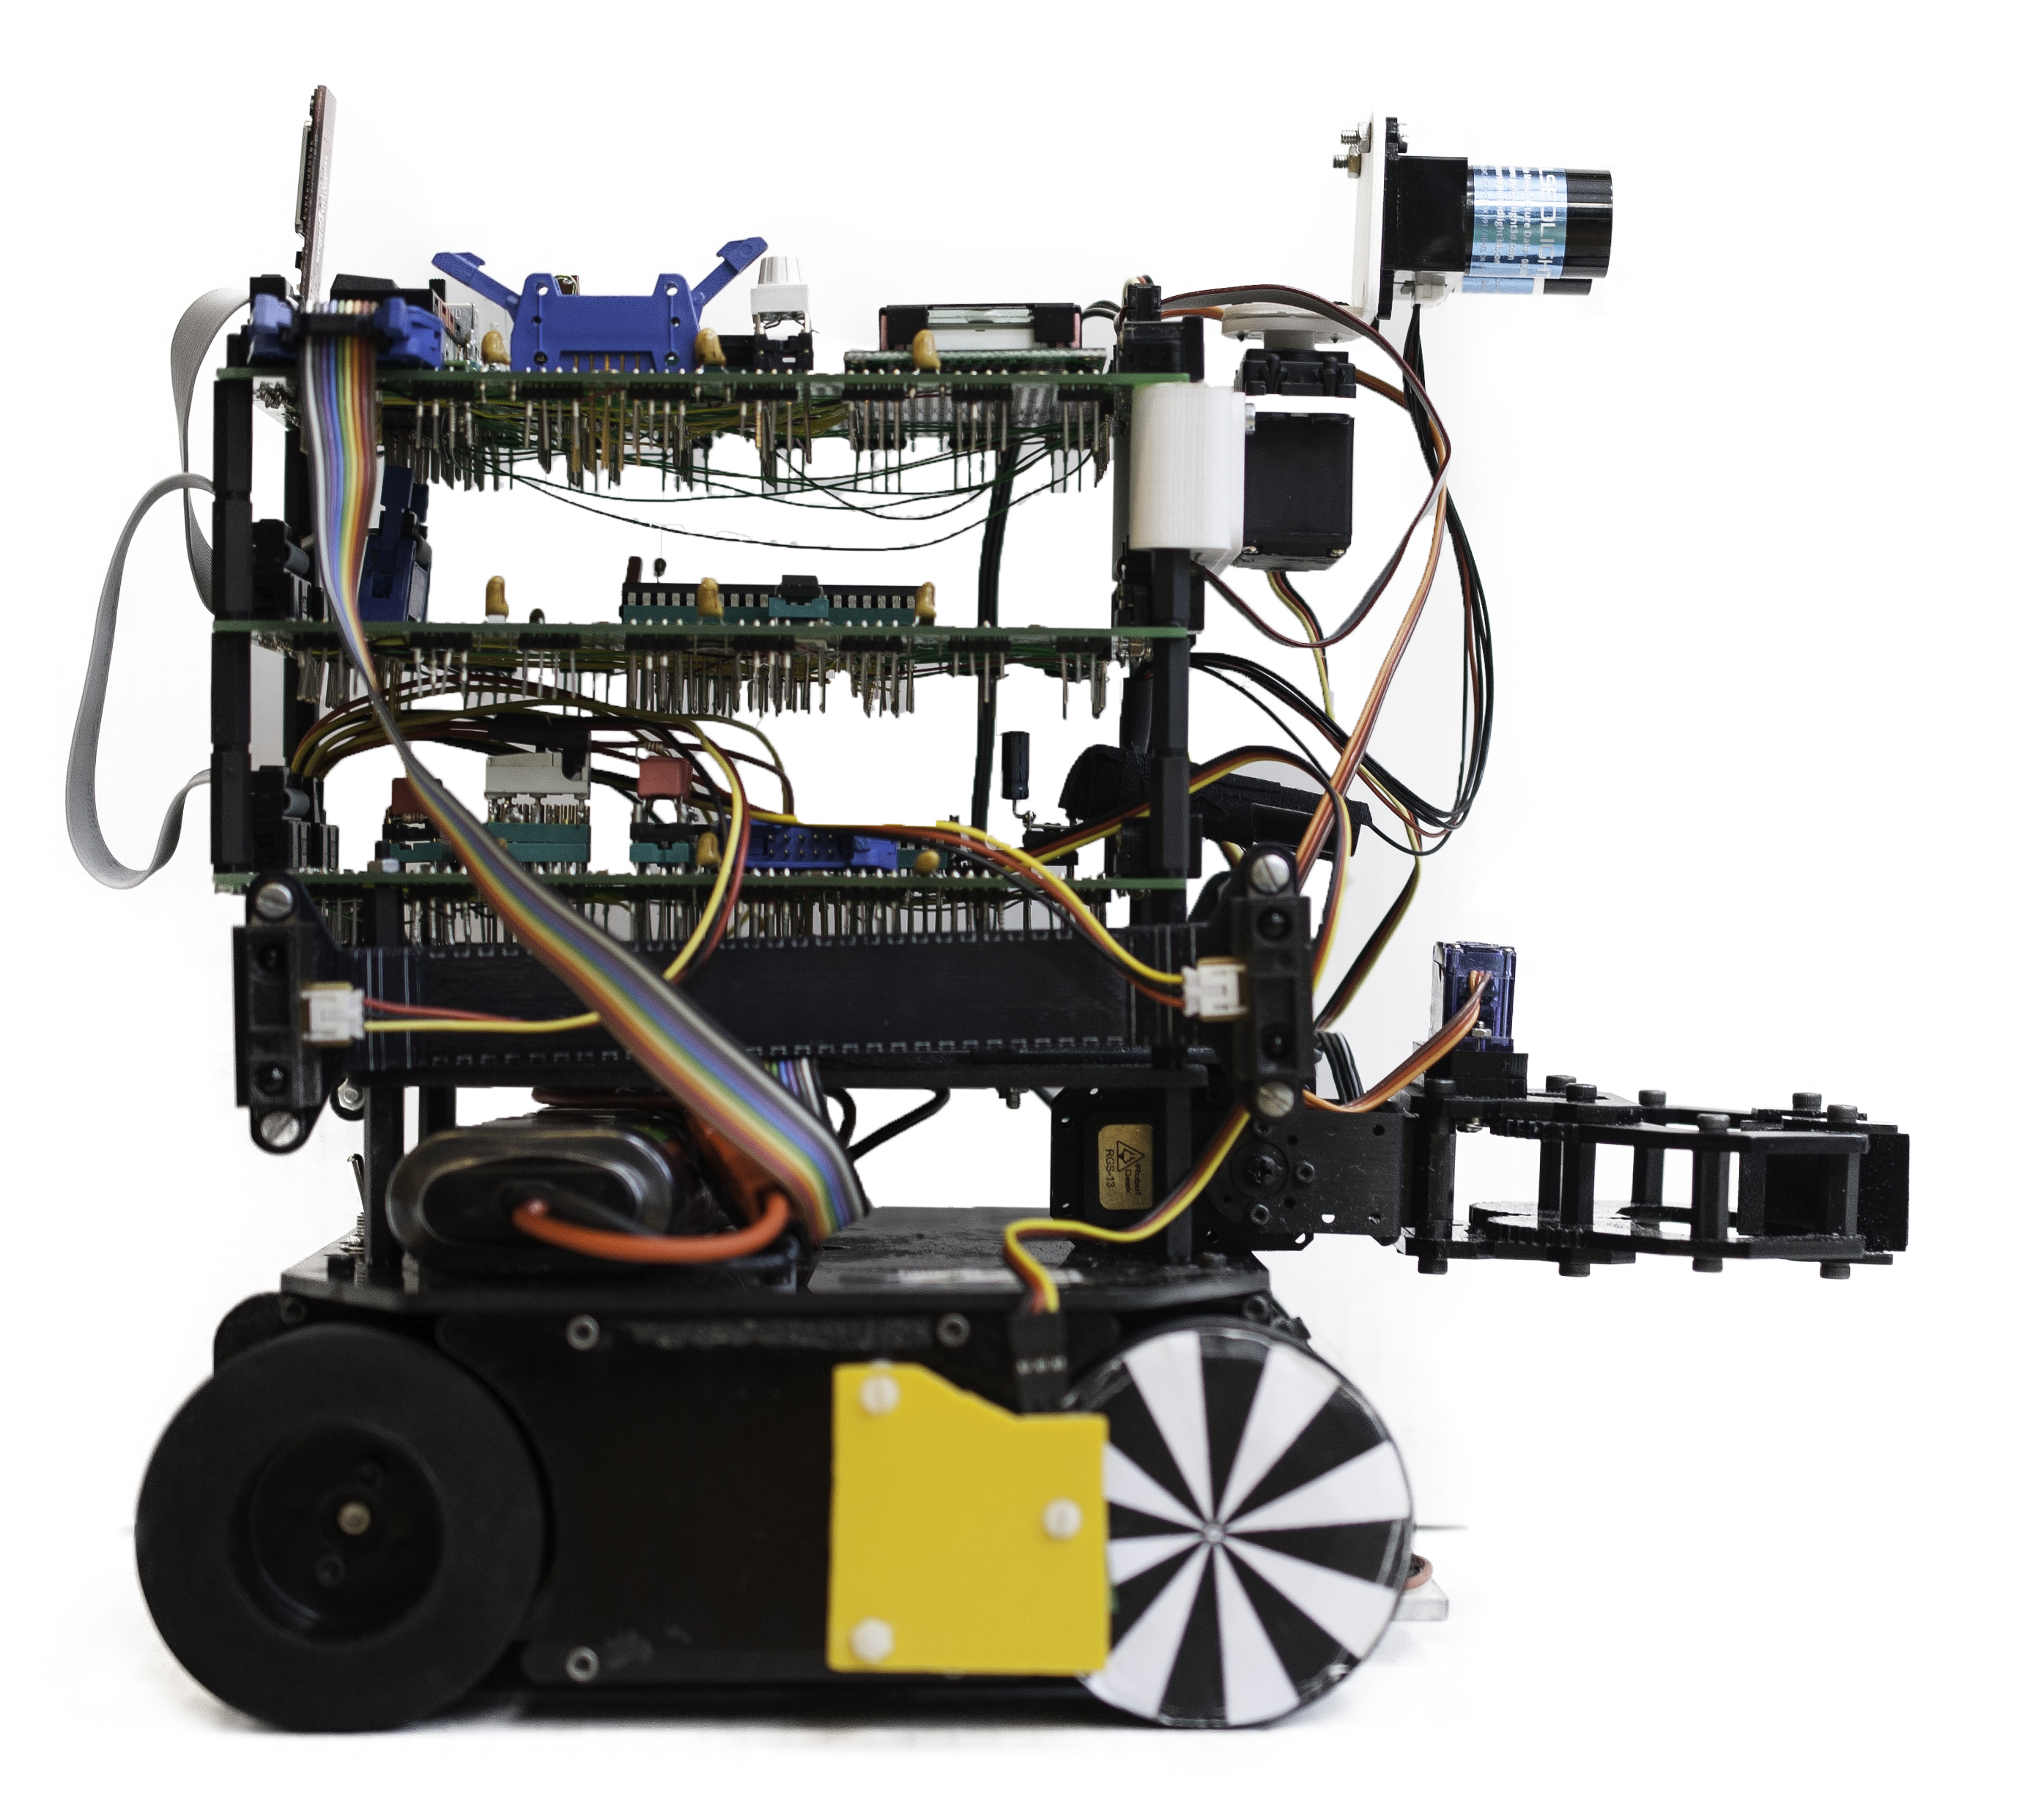
\includegraphics[width=\textwidth]{images/RobotSide.pdf}
    \end{column}
  \end{columns}
\end{frame}

\begin{frame}{Första sliden}
  \begin{itemize}
    \item[-] Bla bla bla
      \pause
    \item[-] Flera saker
      \pause
  \end{itemize}
\end{frame}

\end{document}


